\documentclass{beamer}

\usepackage{graphicx,wrapfig,lipsum}
\usepackage[utf8]{inputenc}
\usepackage[german]{babel}
\usepackage{csquotes}
\usepackage{fontenc}
\usepackage{float}
\usepackage{textcomp}
\usepackage{lmodern}
\usepackage{listings}
\usepackage{courier}
\usepackage{xcolor}
\usepackage{caption}
\usepackage{xifthen}
\usepackage{algorithmicx}
\usepackage{algpseudocode}
\usepackage{pdfpages}


\usetheme{Montpellier}
%\usetheme{default}

\definecolor{bluekeywords}{rgb}{0,0,1}
\definecolor{greencomments}{rgb}{0,0.5,0}
\definecolor{redstrings}{rgb}{0.64,0.08,0.08}
\definecolor{xmlcomments}{rgb}{0.5,0.5,0.5}
\definecolor{types}{rgb}{0.17,0.57,0.68}

\lstloadlanguages{C++}

\lstset{
  language=C++,
  captionpos=b,
  numbers=none,
  numberstyle=\tiny,
  frame=single,
  showspaces=false,
  showtabs=false,
  tabsize=4,
  showstringspaces=false,
  breaklines=true,
  breakatwhitespace=true,
  commentstyle=\color{greencomments},
  keywordstyle=\color{bluekeywords},
  stringstyle=\color{redstrings},
  basicstyle=\ttfamily\scriptsize,
  morekeywords={
    constexpr,
    int8_t, int16_t, int32_t, int64_t, uint8_t, uint16_t, uint32_t, uint64_t},
  literate=
    {á}{{\'a}}1 {é}{{\'e}}1 {í}{{\'i}}1 {ó}{{\'o}}1 {ú}{{\'u}}1
    {Á}{{\'A}}1 {É}{{\'E}}1 {Í}{{\'I}}1 {Ó}{{\'O}}1 {Ú}{{\'U}}1
    {à}{{\`a}}1 {è}{{\`e}}1 {ì}{{\`i}}1 {ò}{{\`o}}1 {ù}{{\`u}}1
    {À}{{\`A}}1 {È}{{\'E}}1 {Ì}{{\`I}}1 {Ò}{{\`O}}1 {Ù}{{\`U}}1
    {ä}{{\"a}}1 {ë}{{\"e}}1 {ï}{{\"i}}1 {ö}{{\"o}}1 {ü}{{\"u}}1
    {Ä}{{\"A}}1 {Ë}{{\"E}}1 {Ï}{{\"I}}1 {Ö}{{\"O}}1 {Ü}{{\"U}}1
    {â}{{\^a}}1 {ê}{{\^e}}1 {î}{{\^i}}1 {ô}{{\^o}}1 {û}{{\^u}}1
    {Â}{{\^A}}1 {Ê}{{\^E}}1 {Î}{{\^I}}1 {Ô}{{\^O}}1 {Û}{{\^U}}1
    {œ}{{\oe}}1 {Œ}{{\OE}}1 {æ}{{\ae}}1 {Æ}{{\AE}}1 {ß}{{\ss}}1
    {ç}{{\c c}}1 {Ç}{{\c C}}1 {ø}{{\o}}1 {å}{{\r a}}1 {Å}{{\r A}}1
    {€}{{\EUR}}1 {£}{{\pounds}}1
}

\newcommand{\includecode}[3][C++]{
  \ifthenelse{\isempty{#3}}
    {\lstinputlisting{#2}}
    {\lstinputlisting[caption={#3}]{#2}}
}
\newcommand{\includecoderange}[5][C++]{\lstinputlisting[caption={#5},firstline=#3,lastline=#4]{#2}}

\title{Formgedächtnislegierung}
\author[Mehmet Ulrich]{Mehmet Ulrich}
%\institute[BuW]{Bergische Universität Wuppertal}

\begin{document}

\frame{\titlepage}

\begin{frame}
\frametitle{Gliederung}
\tableofcontents[hideallsubsections]
\end{frame}

\section{Grundlagen}

\begin{frame}[t]\frametitle{Gliederung: Grundlagen}
\tableofcontents[
currentsection,
subsectionstyle=show/show/hide
]
\end{frame}

\subsection{Kristallgitter}
\label{grnd:gitter}
\begin{frame}
	Das Kristallgitter in Metallen:
	\begin{itemize}
		\item{Kubisch primitives Gitter (simple cubic)}
		\item{Kubisch raumzentriertes Gitter (body centered cubic)}
		\item{Kubisch flächenzentriertes Gitter (face centered cubic)}
	\end{itemize}
\end{frame}

\section{Formgedächtnislegierungen}

\begin{frame}[t]\frametitle{Gliederung: Formgedächtnislegierungen}
\tableofcontents[
currentsection,
subsectionstyle=show/show/hide
]
\end{frame}

\begin{frame}[c]\frametitle{NITINOL}
	\centering
	Nickel Titanium Naval Ordnance Laboratory.
	\\
	Durch zufall 1958 entdeckt.
\end{frame}


 \label{ergb:01}
 \begin{frame}[c]\frametitle{Beispiel Büroklammer}
	\centering
	\begin{figure}
		\begin{minipage}{0.45\textwidth}
		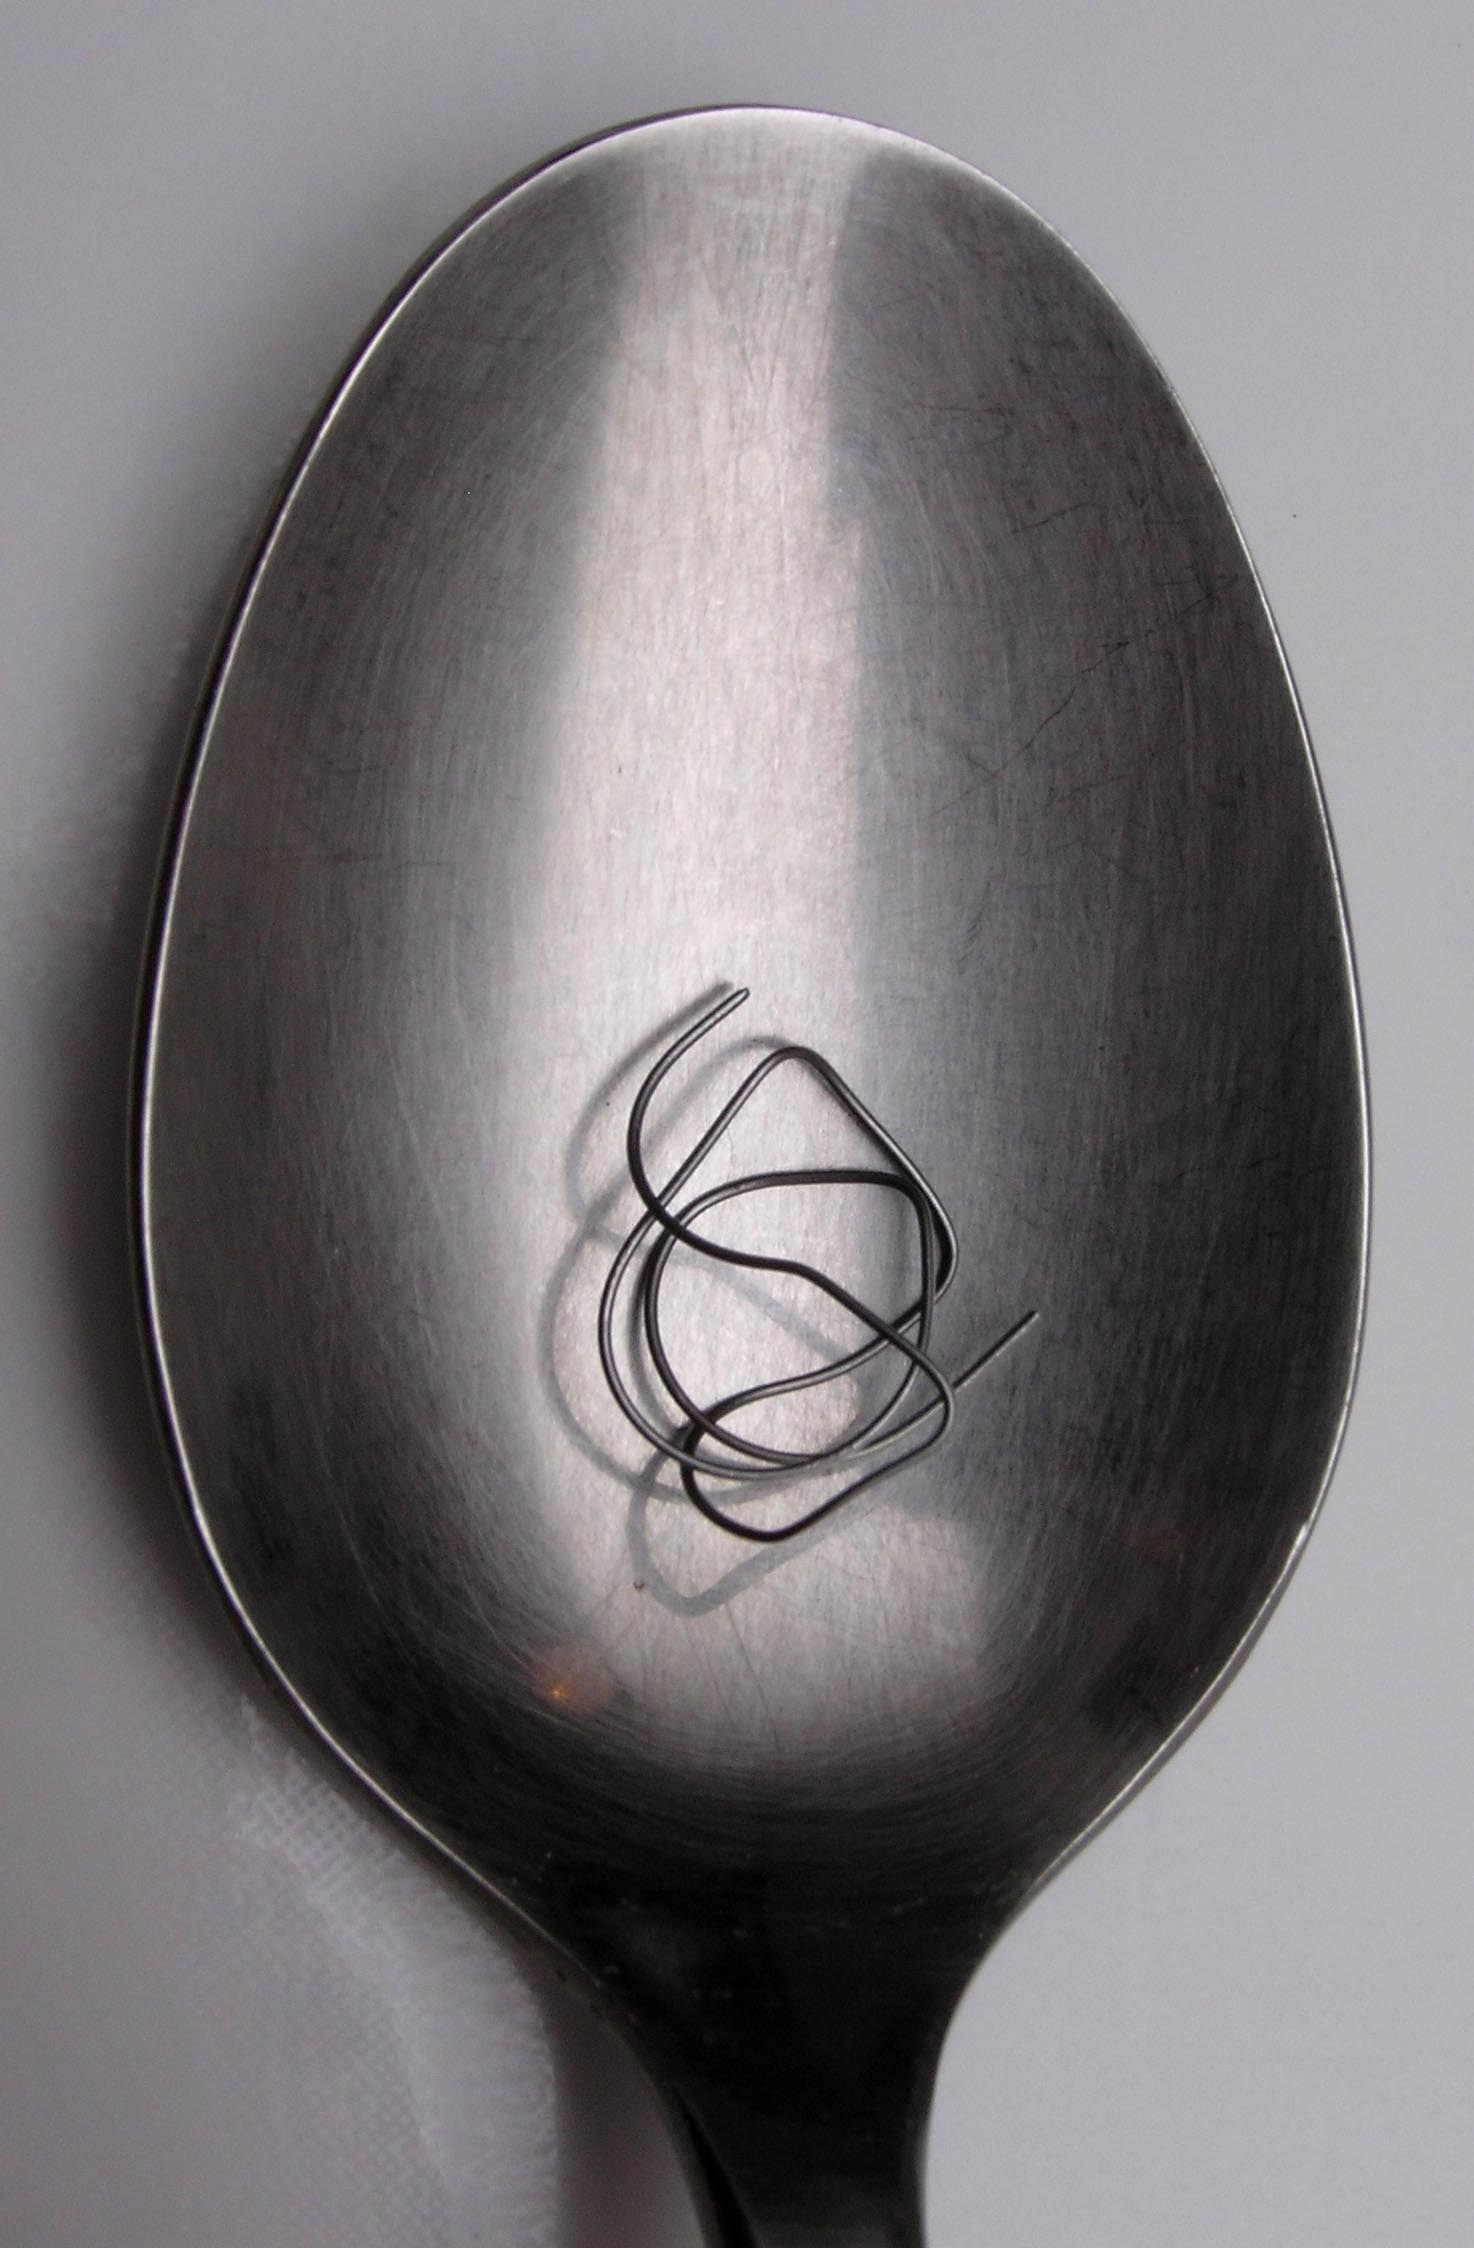
\includegraphics[width=0.5\textwidth]{medien/Nitinol_bueroklammer_verbogen.jpg}
		\end{minipage}
	\hfill
		\begin{minipage}{0.45\textwidth}
		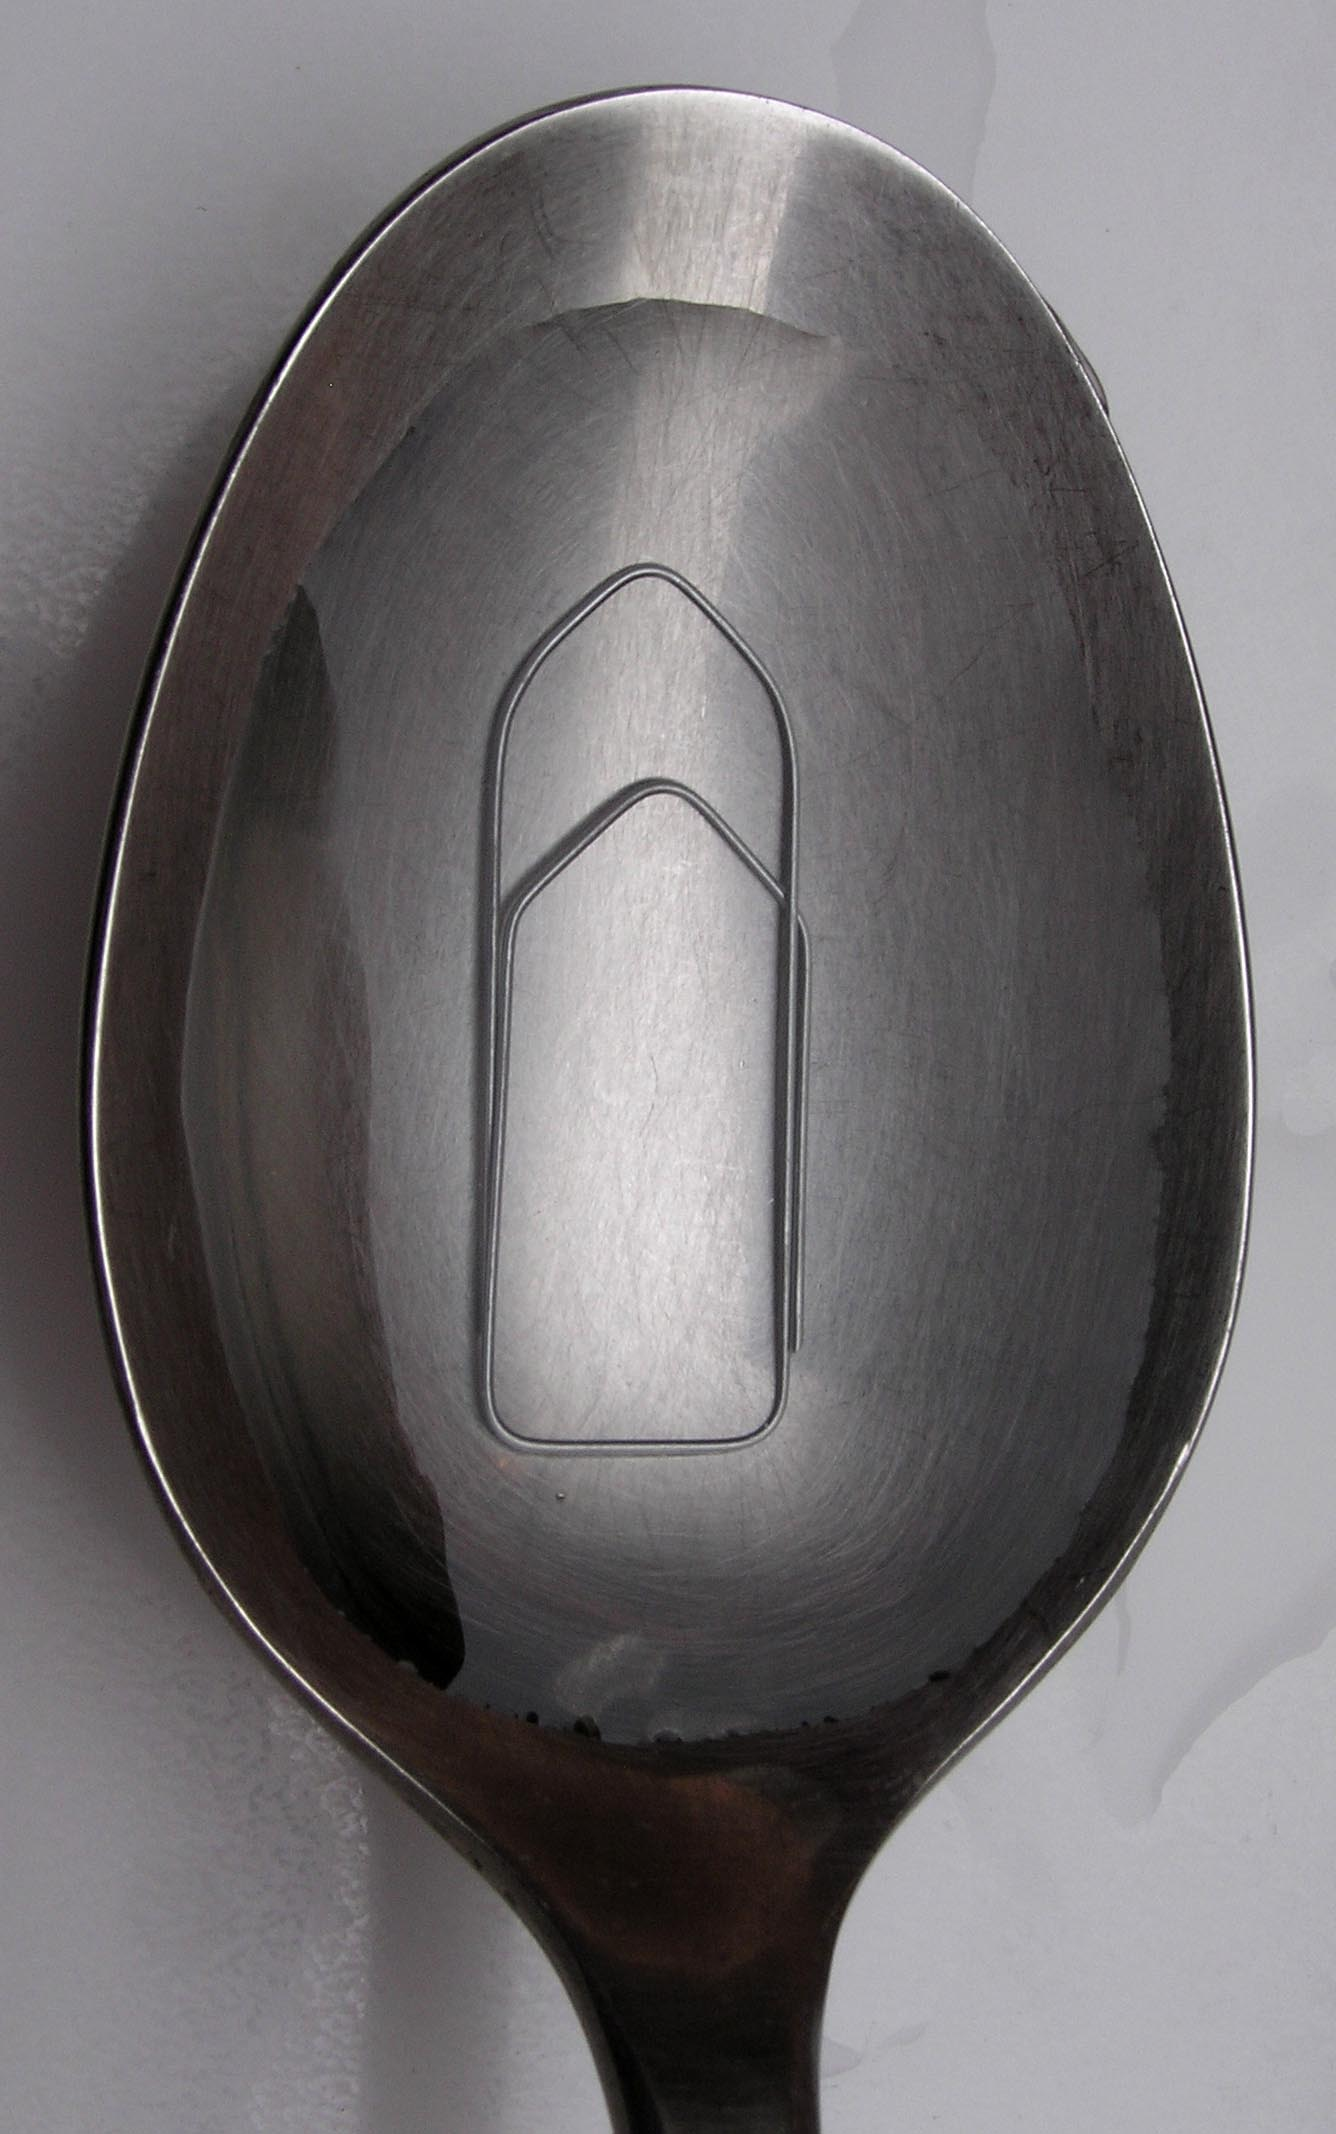
\includegraphics[width=0.5\textwidth]{medien/Nitinol_bueroklammer_heiss.jpg}
		\end{minipage}
	\end{figure}
 \end{frame}

\subsection{Effekte}
\label{fgl:effekte}
\begin{frame}[c]\frametitle{Effekte}
	Verschiedene Effekte von Formgedächtnislegierungen:
	\begin{itemize}
		\item{Einwegeffekt}
		\item{Zweiwegeffekt}
		\item{Pseudoelastizität}
	\end{itemize}
\end{frame}

\subsection{Vergleich}
\begin{frame}[c]\frametitle{Vergleich}
	\centering
	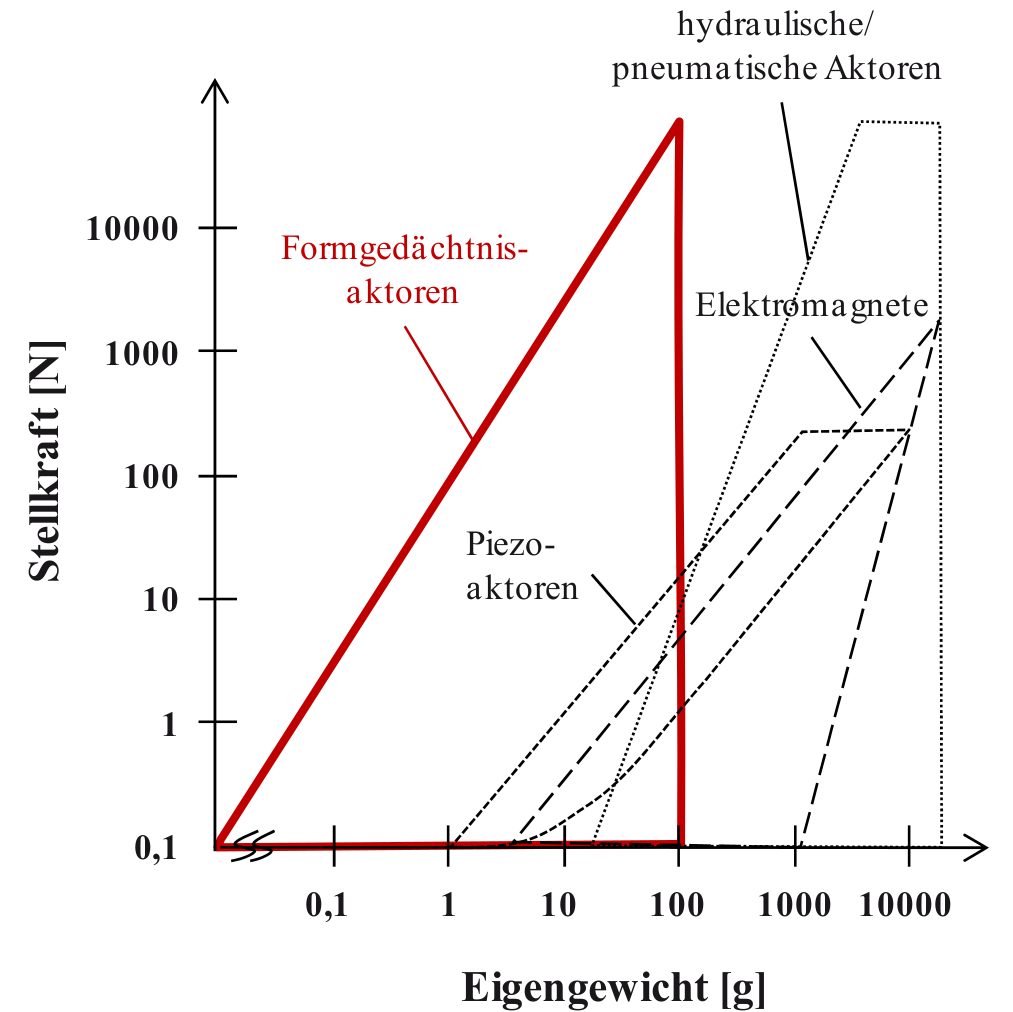
\includegraphics[height=0.5\textwidth]{medien/Verschiedene_Aktorprinzipien.png}
	\\
	\tiny{Quelle: Sven Langbein \& Alexander Czechowicz. Konstruktionspraxis
	Formgedächtnistechnik. Potentiale - Auslegung - Beispiele (Seite: 32).}
\end{frame}

\begin{frame}[c]\frametitle{Temperaturstrahl}
	\centering
	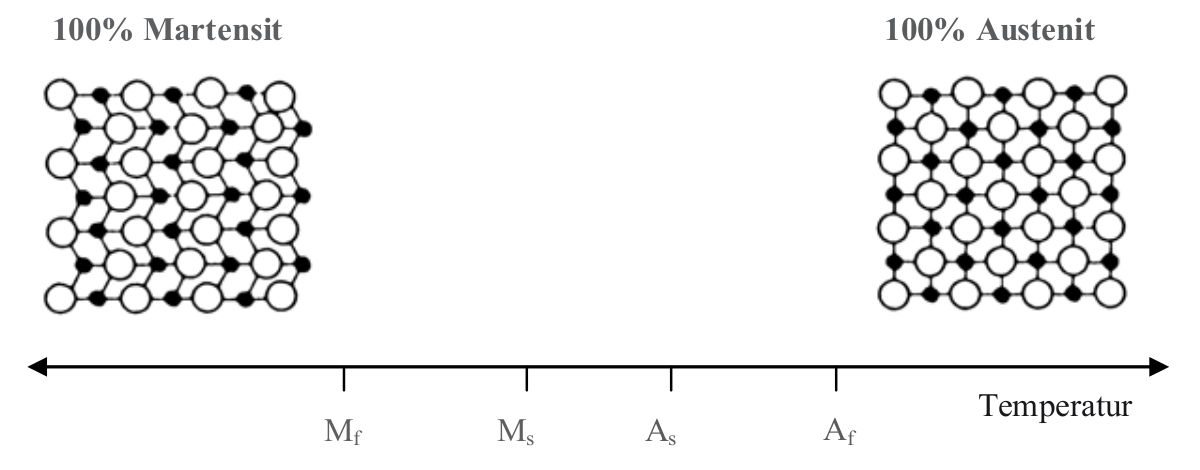
\includegraphics[height=0.35\textwidth]{medien/Umwandlung_anhand_des_Temperaturstrahls.png}
	\\
	\tiny{Quelle: Sven Langbein \& Alexander Czechowicz. Konstruktionspraxis
	Formgedächtnistechnik. Potentiale - Auslegung - Beispiele (Seite: 3).}
\end{frame}

\subsection{Einwegeffekt}
\begin{frame}[t]\frametitle{Einwegeffekt}
	\centering
	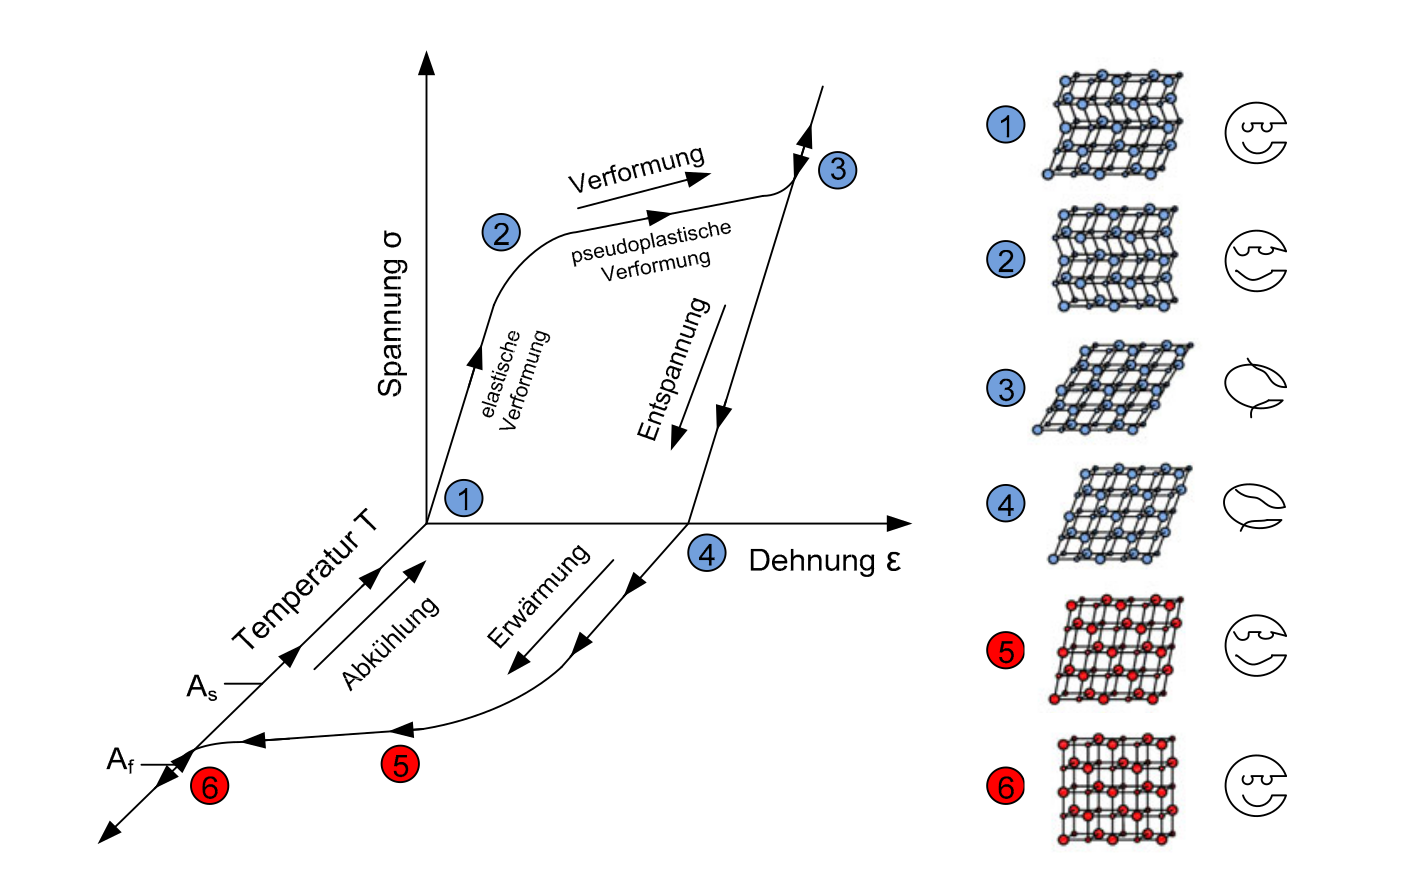
\includegraphics[height=0.5\textwidth]{medien/Verhalten_beim_Einwegeffekt.png}
	\\
	\tiny{Quelle: Sven Langbein \& Alexander Czechowicz. Konstruktionspraxis
	Formgedächtnistechnik. Potentiale - Auslegung - Beispiele (Seite: 6).}
\end{frame}

\subsection{Zweiwegeffekt}
\begin{frame}[t]\frametitle{Zweiwegeffekt}
	\centering
	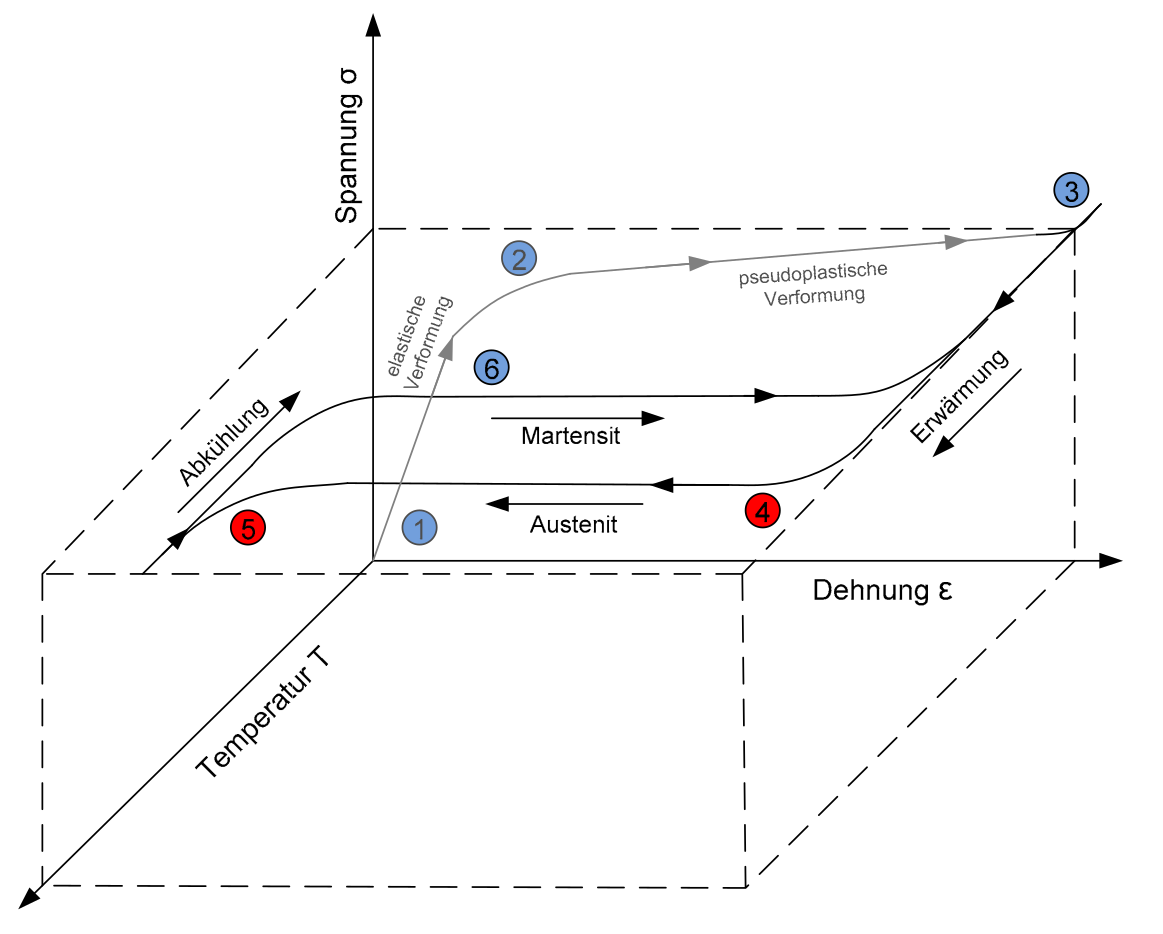
\includegraphics[height=0.5\textwidth]{medien/Verhalten_beim_Zweiwegeffekt.png}
	\\
	\tiny{Quelle: Sven Langbein \& Alexander Czechowicz. Konstruktionspraxis
	Formgedächtnistechnik. Potentiale - Auslegung - Beispiele (Seite: 7).}
\end{frame}

\subsection{Pseudoelastizität}
\begin{frame}[c]\frametitle{Pseudoelastizität}
	Die Umwandlungstemperatur liegt unter der Arbeitstemperatur
	(Umgebugstemperatur), im Normalfall unter 0°C.\\
	\centering
	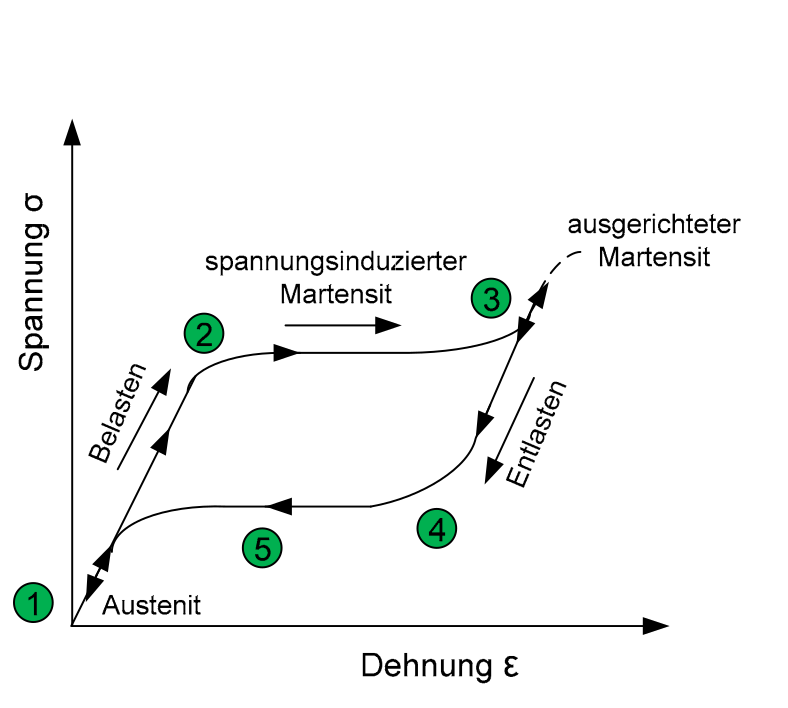
\includegraphics[height=0.5\textwidth]{medien/Verhalten_beim_pseudoelastischen_Effekt.png}
	\\
	\tiny{Quelle: Sven Langbein \& Alexander Czechowicz. Konstruktionspraxis
	Formgedächtnistechnik. Potentiale - Auslegung - Beispiele (Seite: 8).}
\end{frame}

\begin{frame}[c]\frametitle{Widerstandsänderung}
	\centering
	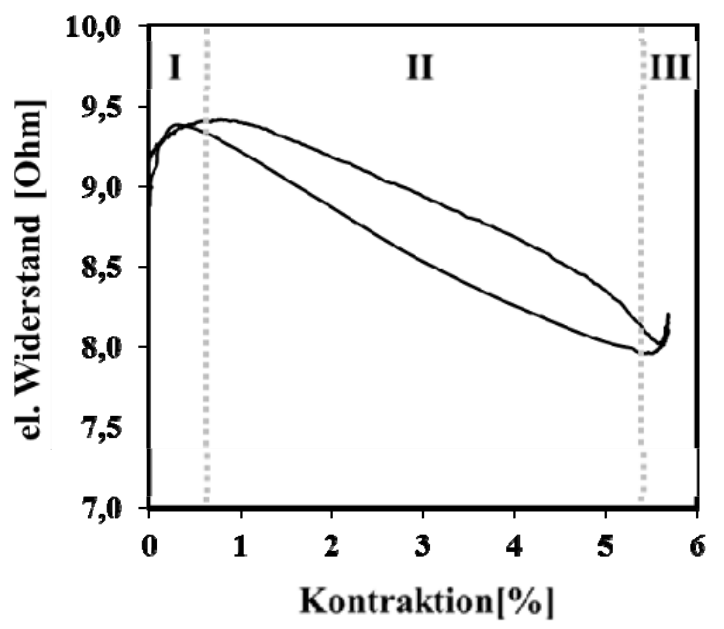
\includegraphics[height=0.5\textwidth]{medien/widerstand_zu_kontraktion.png}
	\\
	\tiny{Quelle: Sven Langbein \& Alexander Czechowicz. Konstruktionspraxis
	Formgedächtnistechnik. Potentiale - Auslegung - Beispiele (Seite: 110).}
\end{frame}

\subsection{Nutzbare FGL}
\begin{frame}[c]\frametitle{Nutzbare FGL}
	\centering
	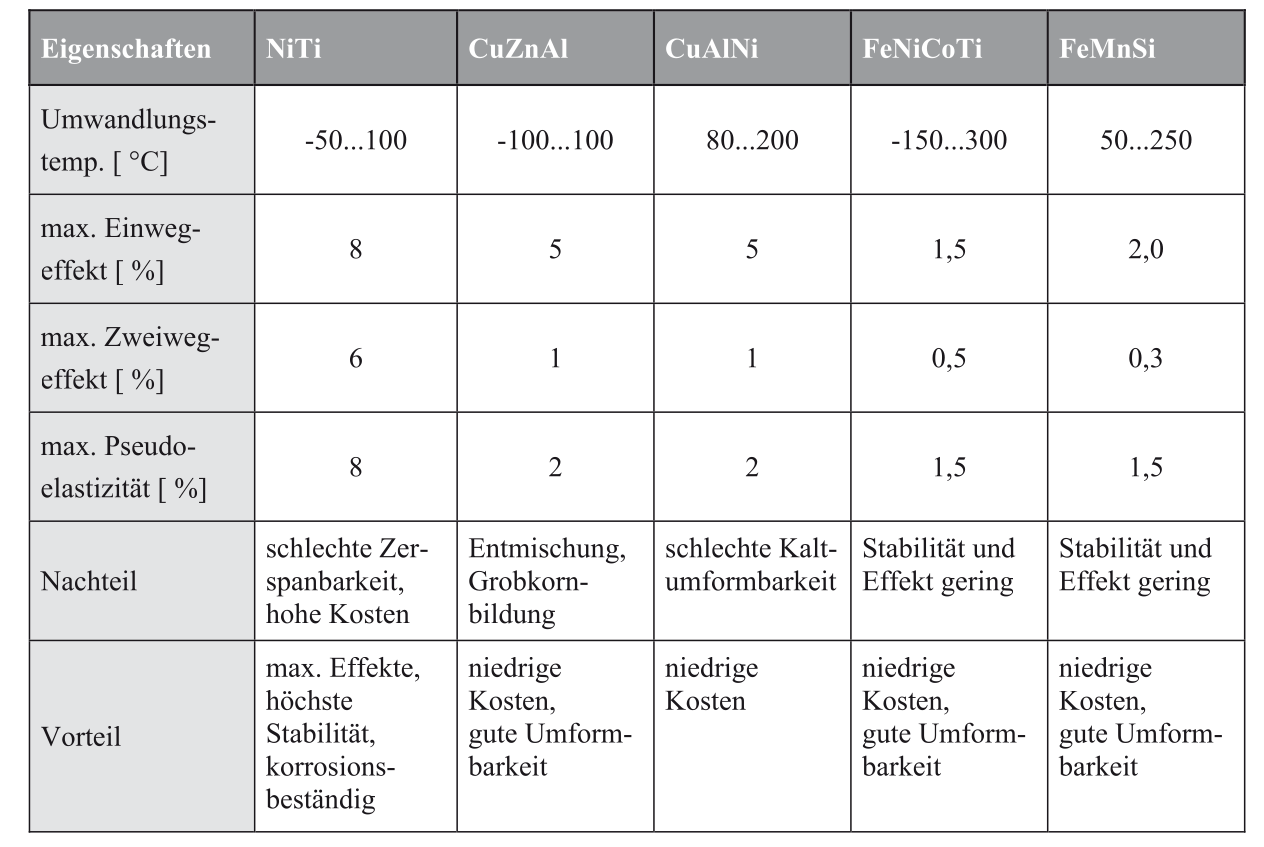
\includegraphics[height=0.5\textwidth]{medien/fgl_tabelle.png}
	\\
	\tiny{Quelle: Sven Langbein \& Alexander Czechowicz. Konstruktionspraxis
	Formgedächtnistechnik. Potentiale - Auslegung - Beispiele (Seite: 9).}
\end{frame}

\section{Warum FGL}

\begin{frame}[t]\frametitle{Gliederung: Warum FGL}
\tableofcontents[
currentsection,
subsectionstyle=show/show/hide
]
\end{frame}

\subsection{Warum FGL}
\label{thesis}
\begin{frame}[c]\frametitle{Warum FGL}
	Warum FGL
	\begin{itemize}
		\item{Arbeit als Studentische Hilfskraft}
		\item{Noch zu lösende Probleme }
		\item{Neue Forschungsansätze und anfrage einer Thesis}
	\end{itemize}
\end{frame}

\subsection{Was habe ich gemacht}
\label{eigenearbeit}
\begin{frame}[c]\frametitle{Ziel}
Hinderniserkennung mit Widerstandsänderung des FGL
\end{frame}

\begin{frame}
	\begin{itemize}
		\item{Messen des Leitwerts wärend des Bestromens}
		\item{Software entwickeln welche ein Hindernis erkennt}
	\end{itemize}
\end{frame}

\end{document}
